\documentclass{beamer}
\usepackage[utf8]{inputenc}
\usepackage{mystyle} % See mystyle.sty for packages and own commands
%------------------------------------------------------------
%Title page
\title[Solving Nonlinear Equations]{Solving Nonlinear Equations \small{(using python)}}
\subtitle{Assignment 1}
\titlegraphic{
\includegraphics[height=0.85cm]{Logos/iitmlogo.png}}
\author[Gaddam Shiva Kumar]{Gaddam Shiva Kumar (MM22D014)}
\institute[]{ME7227 : Nonlinear Finite Element Analysis of Solid Continua}
\date{\today}

%---------------------TITLE PAGE---------------------------------------
\begin{document}
\begin{frame}
\maketitle
\end{frame}
%------------------------------------------------------------

% \logo{
\includegraphics[height=1cm]{Logos/circlelogo.png}~%
% }


%===================================================================
\section{Introduction}

% \begin{frame}
% \frametitle{Table of Contents}
% \tableofcontents
% \end{frame}

\begin{frame}{Introduction}{Steps involved in solving a nonlinear single-variable equation}
    \begin{columns}
        \column{0.9\textwidth}
        \begin{block}{\footnotesize Let $F(x)=f$ be a nonlinear equation where $F(x)$ is a nonlinear function in variable `x'.}
            \begin{enumerate}
                \footnotesize
                \item Start with an initial guess `$x_0$'
                \item Linearize the function $F(x)$ at `$x_0$' using Taylor series expansion.
                \[
                    F(x)\approx F_L(x)=\big(F(x_0)-F'(x_0) x_0\big)+F'(x_0) x
                \]
                \item Solve for the solution(say $x^*$) using the linearized equation $F_L(x^*)=f$.
                \item Compute the relative error in `f' i.e.
                \[
                    \text{rel. error} = \frac{f-f^*}{f} = \frac{f-F(x^*)}{f}
                \]
                \item if the relative error is with in the required tolerance, obtained $x^*$ is the solution. Otherwise, replace initial guess with the $x^*$ and repeat steps 2 to 5.
            \end{enumerate}
        \end{block}
    \end{columns}
    \vfill
\end{frame}

%===================================================================
\section{Problem 1}

\begin{frame}{Problem 1}{Plotting the function}
    \vspace{-3em}
    \begin{columns}
        \column[t]{0.47\textwidth}
        \begin{block}{\footnotesize The nonlinear equation}
            \footnotesize
            \[F(x)=\frac{x}{\sin x}=f\]
            \begin{itemize}
                \item Oscillatory in nature
                \item Multiple solutions are possible for a given 'f'
            \end{itemize}
        \end{block}
        \column[t]{0.47\textwidth}
        \begin{block}{\footnotesize Plot of the nonlinear function}
            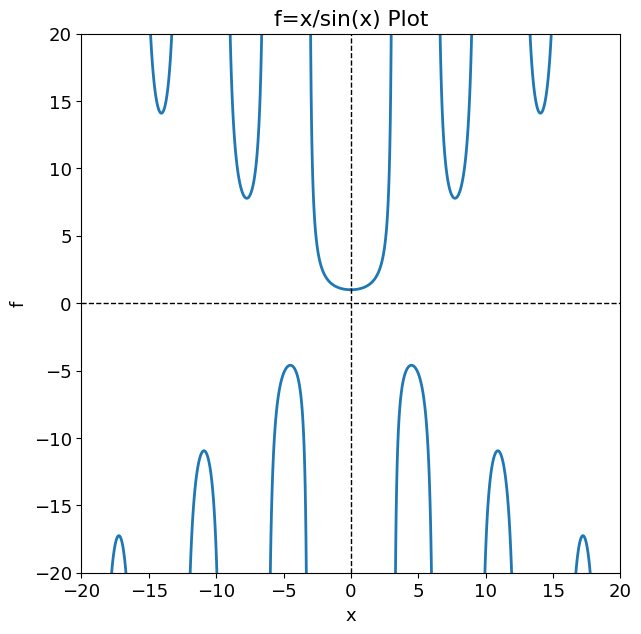
\includegraphics[width=\textwidth]{Figures/prob1_functionplot.png}
        \end{block}
    \end{columns}
\end{frame}

\begin{frame}{Problem 1}{Solution at 'f' = 1.2, Case:1}
    \begin{block}{\footnotesize Initial guess = 2.5, f = 1.2}
        \footnotesize
        Solution is : x = 1.026738, Corresponding 'f' = 1.200000, No of iterations = 6
    \end{block}
    \vspace{-0.5em}
    \begin{columns}
        \column{0.43\textwidth}
        \begin{block}{}
            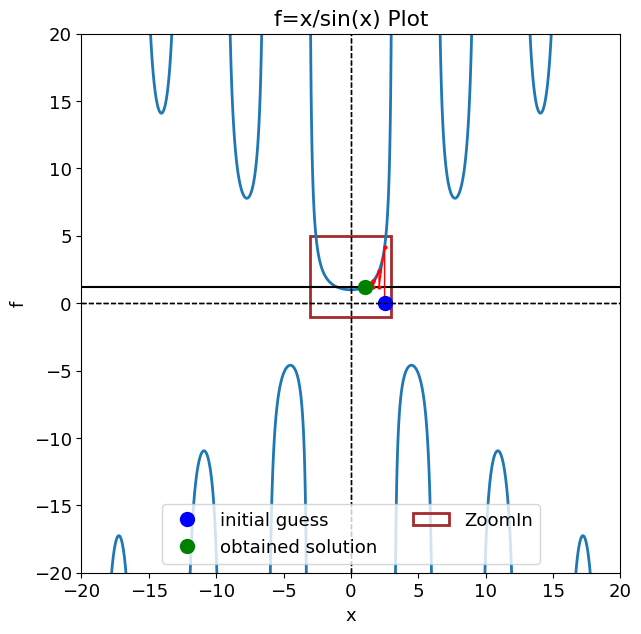
\includegraphics[width=\textwidth]{Figures/prob1_sol11.png}
        \end{block}
        \column{0.07\textwidth}
        \[\implies\]
        \column{0.42\textwidth}
        \begin{block}{}
            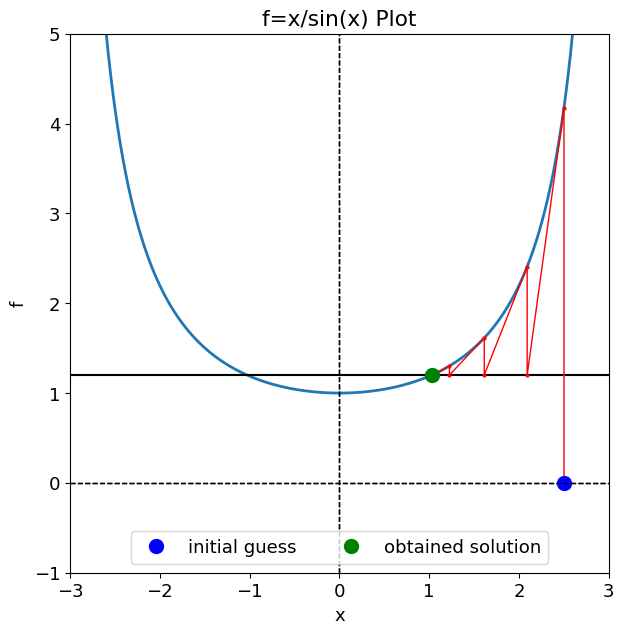
\includegraphics[width=\textwidth]{Figures/prob1_sol12.png}
        \end{block}
    \end{columns}
\end{frame}

\begin{frame}{Problem 1}{Solution at 'f' = 1.2, Case:2}
    \begin{block}{\footnotesize Initial guess = 0.1001, f = 1.2}
        \footnotesize
        Solution is : x = 1.026738, Corresponding 'f' = 1.200000, No of iterations = 33
    \end{block}
    \vspace{-0.5em}
    \begin{columns}
        \column{0.43\textwidth}
        \begin{block}{}
            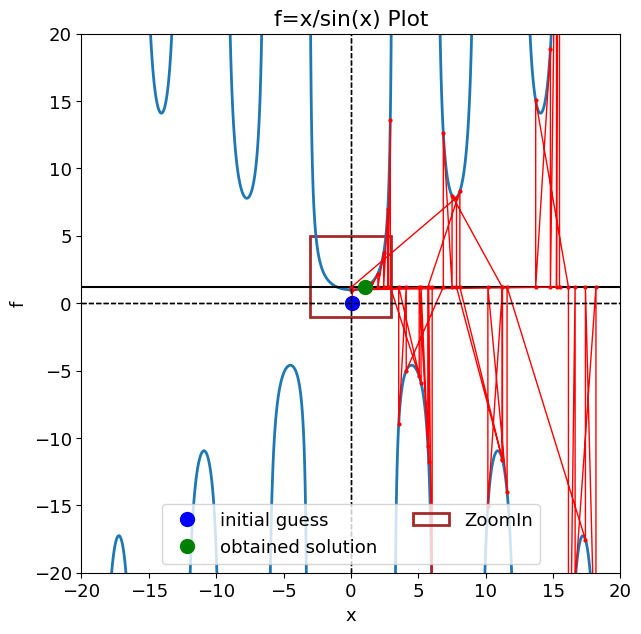
\includegraphics[width=\textwidth]{Figures/prob1_sol21.png}
        \end{block}
        \column{0.07\textwidth}
        \[\implies\]
        \column{0.42\textwidth}
        \begin{block}{}
            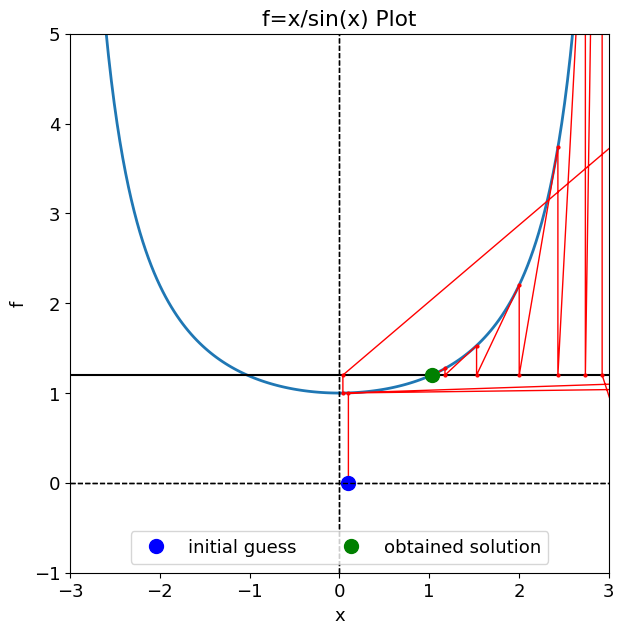
\includegraphics[width=\textwidth]{Figures/prob1_sol22.png}
        \end{block}
    \end{columns}
\end{frame}

\begin{frame}{Problem 1}{Solution at 'f' = 1.2, Case:3}
    \begin{block}{\footnotesize Initial guess = 0.1000, f = 1.2}
        \footnotesize
        Maximum allowed no of iterations(200) reached.
    \end{block}
    \vspace{-1.5em}
    \begin{columns}
        \column[t]{0.46\textwidth}
        \begin{block}{}
            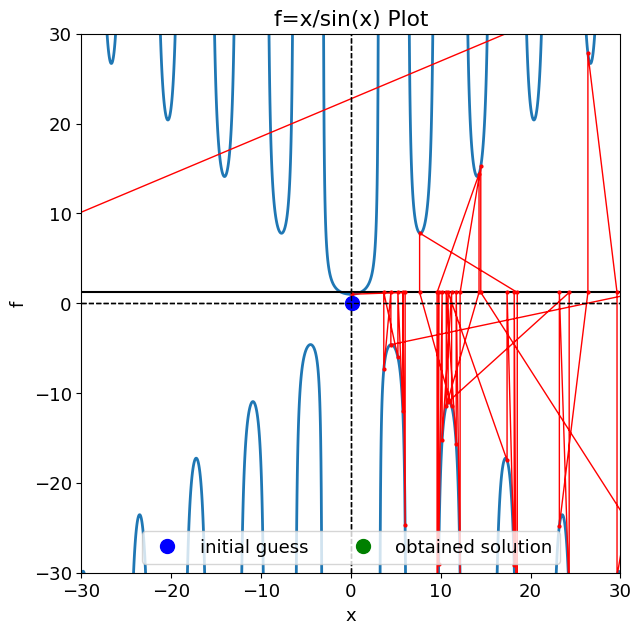
\includegraphics[width=\textwidth]{Figures/prob1_sol31.png}
        \end{block}
        \column[t]{0.46\textwidth}
        \begin{block}{\footnotesize Observations}
            \footnotesize
            \begin{itemize}
                \item From the previous test cases it can be observed that when the initial guess is in the neighborhood of solution, it will most probably converge. 
                \item It is also observed that when the initial guess is far away from solution, it may or may not converge.
            \end{itemize}
        \end{block}
    \end{columns}
\end{frame}

\begin{frame}{Problem 1}{Solution at 'f' = 10}
    \vspace{-2.5em}
    \begin{columns}
        \column[t]{0.43\textwidth}
        \begin{table}
            \centering
            \footnotesize
            \begin{tabular}{cc}
                \toprule
                Initial Guess & Solution \\
                \midrule
                6.5     &   7.068174 \\
                3.13    &   2.852342 \\
                -4      &  -8.423204 \\
                \bottomrule
            \end{tabular}
        \end{table}
        \begin{block}{\footnotesize Observations}
            \footnotesize
            \begin{itemize}
                \item In case of multiple solutions, the obtained solution really depends on the initial guess.
                \item It could be either the one in the neighborhood of initial guess or something completely arbitrary.
            \end{itemize}
        \end{block}
        \column[t]{0.5\textwidth}
        \begin{block}{}
            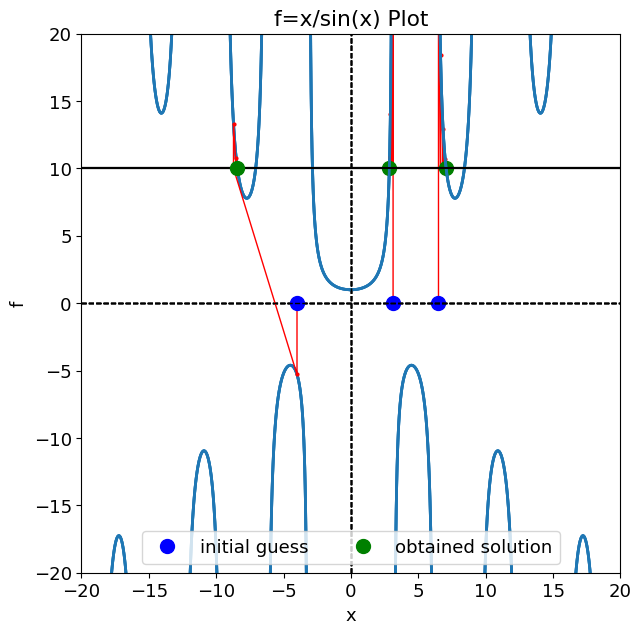
\includegraphics[width=\textwidth]{Figures/prob1_sol41.png}
        \end{block}
    \end{columns}
\end{frame}

\begin{frame}{Problem 1}{Plotting the solution curve, $f\in[-20,20]$}
    \vspace{-2.5em}
    \begin{columns}
        \column[t]{0.5\textwidth}
        \begin{block}{\footnotesize Depends on initial guess (3.12, -1.5)}
            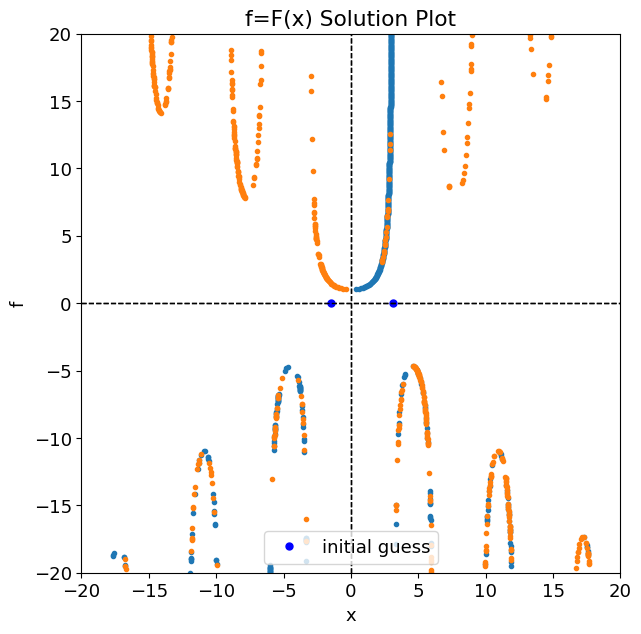
\includegraphics[width=\textwidth]{Figures/prob1_pltsol1.png}
        \end{block}
        \column[t]{0.43\textwidth}
        \begin{block}{\footnotesize Observations }
            \footnotesize
            \begin{itemize}
                \item For a grid of 1000 points on 'f' axis, and with an arbitrary initial guess the graph plotted gives an incomplete description of the nonlinear function.
                \item But by carefully choosing the initial guess one could be able to plot any monotonic section of the plot.
            \end{itemize}
        \end{block}
    \end{columns}
\end{frame}

\begin{frame}{Problem 1}{Plotting the solution curve, $f\in[-20,20]$}
    \vspace{-2.5em}
    \begin{columns}
        \column[t]{0.5\textwidth}
        \begin{block}{\footnotesize For multiple initial guesses - combined plot}
            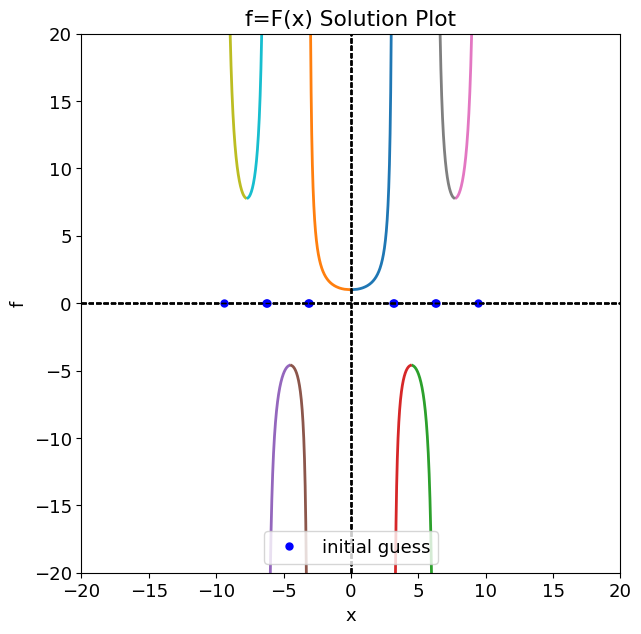
\includegraphics[width=\textwidth]{Figures/prob1_pltsol2.png}
        \end{block}
        \column[t]{0.43\textwidth}
        \begin{block}{\footnotesize Observations }
            \footnotesize
            \begin{itemize}
                \item For a grid of 1000 points on 'f' axis, and with an arbitrary initial guess the graph plotted gives an incomplete description of the nonlinear function.
                \item But by carefully choosing the initial guess one could be able to plot any monotonic section of the graph.
                \item And with many such initial guesses it is possible to get complete description of the nonlinear function.
            \end{itemize}
        \end{block}
    \end{columns}
\end{frame}

% \begin{frame}{Problem 1}{Plotting the solution curve, $f\in[-20,20]$}
%     \vspace{-2.5em}
%     \begin{columns}
%         \column[t]{0.45\textwidth}
%         \begin{block}{\scriptsize Depends on initial guess (3.12, -1.5)}
%             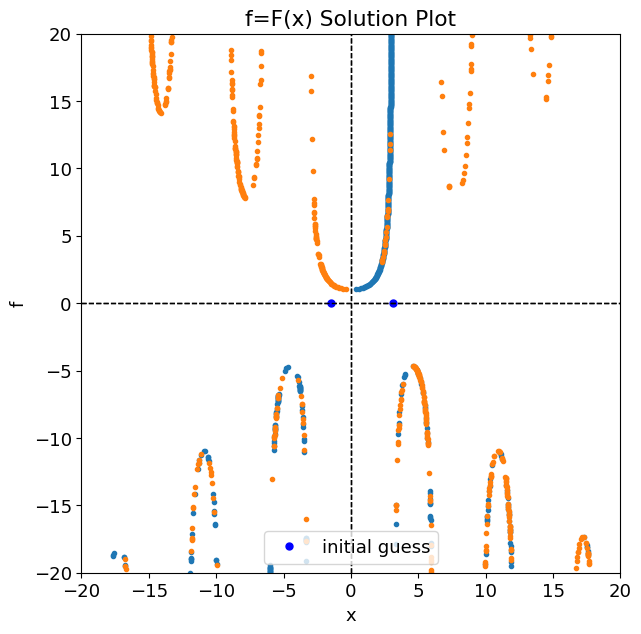
\includegraphics[width=\textwidth]{Figures/prob1_pltsol1.png}
%         \end{block}
%         \column[t]{0.45\textwidth}
%         \begin{block}{\scriptsize For multiple initial guesses - combined plot }
%             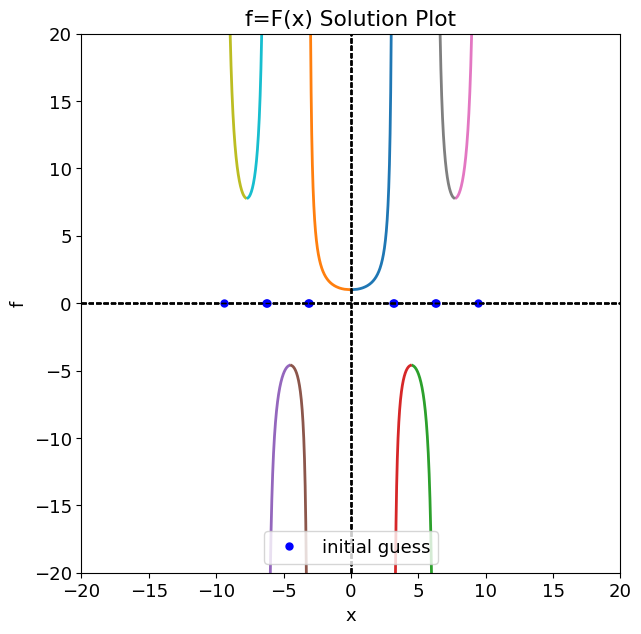
\includegraphics[width=\textwidth]{Figures/prob1_pltsol2.png}
%         \end{block}
%     \end{columns}
%     \begin{block}{}
        
%     \end{block}
% \end{frame}

%===================================================================
\section{Problem 2}

\begin{frame}{Problem 2}{Plotting the function}
    \vspace{-0.7em}
    \begin{columns}
        \column{0.88\textwidth}
        \begin{block}{\footnotesize The function}
            \scriptsize
            $\displaystyle F(x)\ =\ \frac{1}{15}\sum_{k=0}^{n}\left(-1\right)^{k}\left(\frac{\left(2n+1\right)!}{\left(2n-2k\right)!\left(2k+1\right)!}\right)\left(1-x^{2}\right)^{\left(n-k\right)}\cdot x^{2k} = f, \quad n=9$
        \end{block}
    \end{columns}
    \vspace{-0.3em}
    \begin{columns}
        \footnotesize
        \column[t]{0.4\textwidth}
        \begin{block}{\footnotesize Plotted using python}
            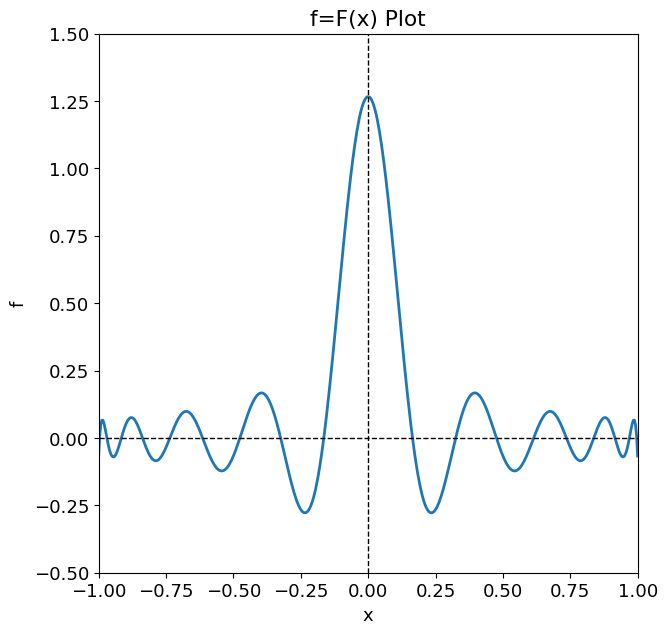
\includegraphics[width=\textwidth]{Figures/prob2_functionplot.png}
        \end{block}
        \column[t]{0.4\textwidth}
        \begin{block}{\footnotesize Verified using Desmos}
            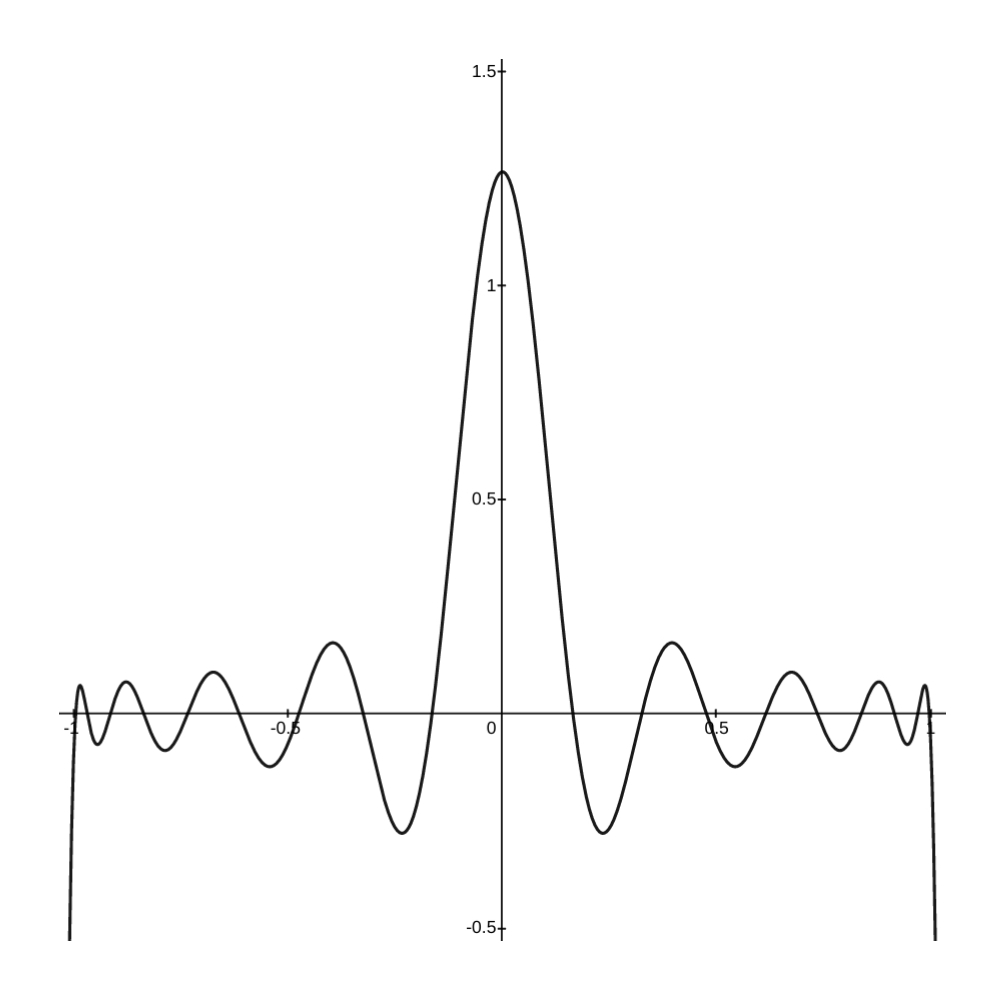
\includegraphics[width=\textwidth, trim={0 0.8cm 0 0.8cm}, clip]{Figures/prob2_functionplotdesmos2.jpg}
        \end{block}
    \end{columns}
\end{frame}

\begin{frame}{Problem 2}{Solution at 'f' = 0.0001}
    \vspace{-2em}
    \begin{columns}
        \column[t]{0.45\textwidth}
        \begin{block}{\footnotesize Initial guess = 0.01, f = 0.0001}
            \footnotesize
            Solution is : x = 0.837203
        \end{block}
        \column[t]{0.45\textwidth}
        \begin{block}{\footnotesize Initial guess = -0.7, f = 0.0001}
            \footnotesize
            Solution is : x = -0.735685
        \end{block}
    \end{columns}
    \vspace{-0.3em}
    \begin{columns}
        \column[t]{0.45\textwidth}
        \begin{block}{}
            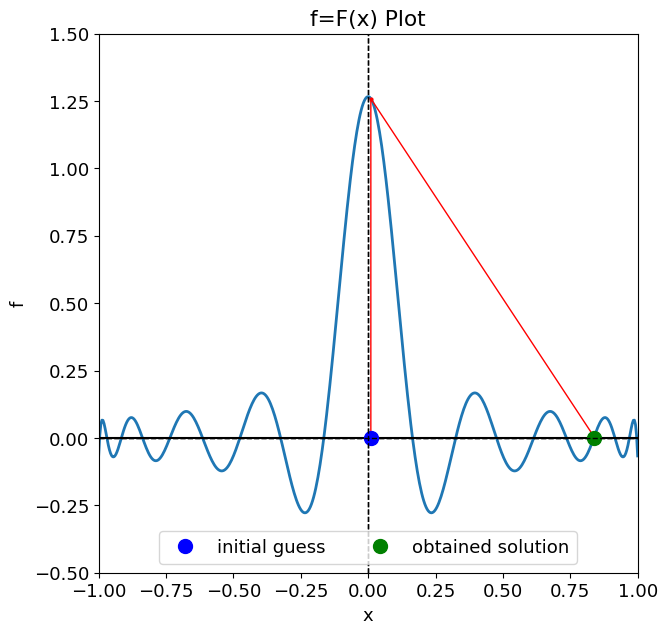
\includegraphics[width=\textwidth]{Figures/prob2_sol11.png}
        \end{block}
        \column[t]{0.45\textwidth}
        \begin{block}{}
            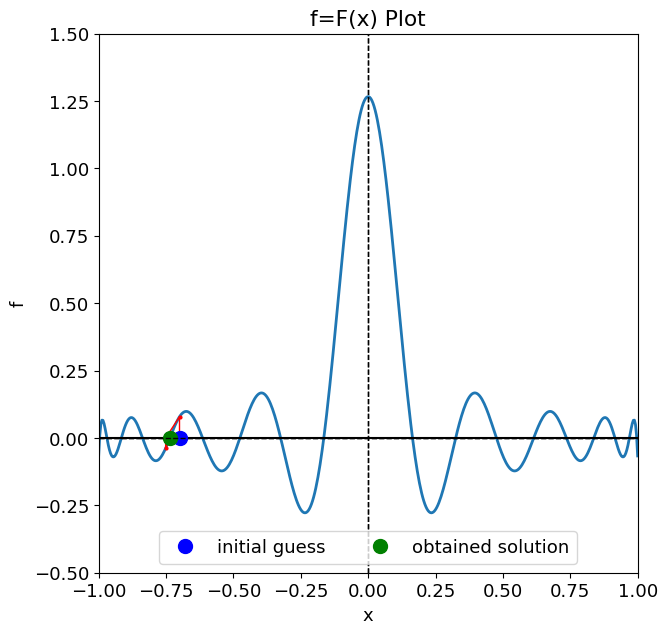
\includegraphics[width=\textwidth]{Figures/prob2_sol12.png}
        \end{block}
    \end{columns}
\end{frame}

\begin{frame}{Problem 2}{Solution at 'f' = 0.25}
    \vspace{-2em}
    \begin{columns}
        \column[t]{0.45\textwidth}
        \begin{block}{\footnotesize Initial guess = 0.033, f = 0.25}
            \footnotesize
            Solution is : x = -0.136611
        \end{block}
        \column[t]{0.45\textwidth}
        \begin{block}{\footnotesize Initial guess = 0.032, f = 0.25}
            \footnotesize
            Maximum iterations reached - 200
        \end{block}
    \end{columns}
    \vspace{-0.3em}
    \begin{columns}
        \column[t]{0.45\textwidth}
        \begin{block}{}
            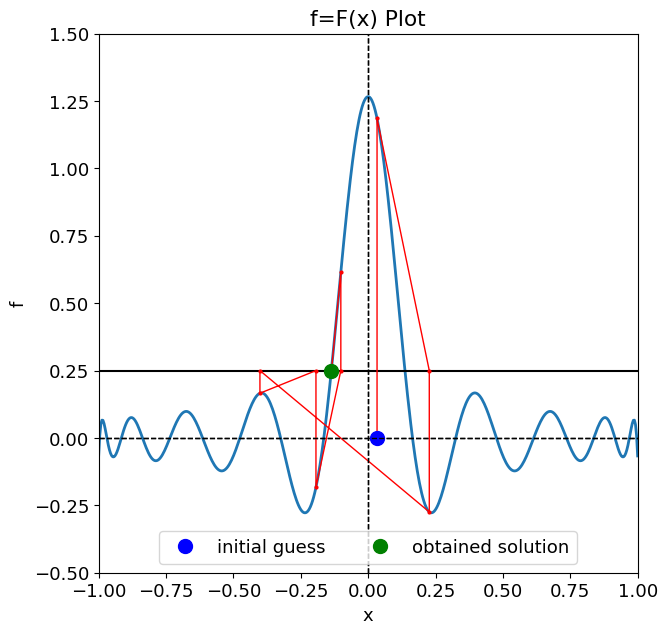
\includegraphics[width=\textwidth]{Figures/prob2_sol21.png}
        \end{block}
        \column[t]{0.45\textwidth}
        \begin{block}{}
            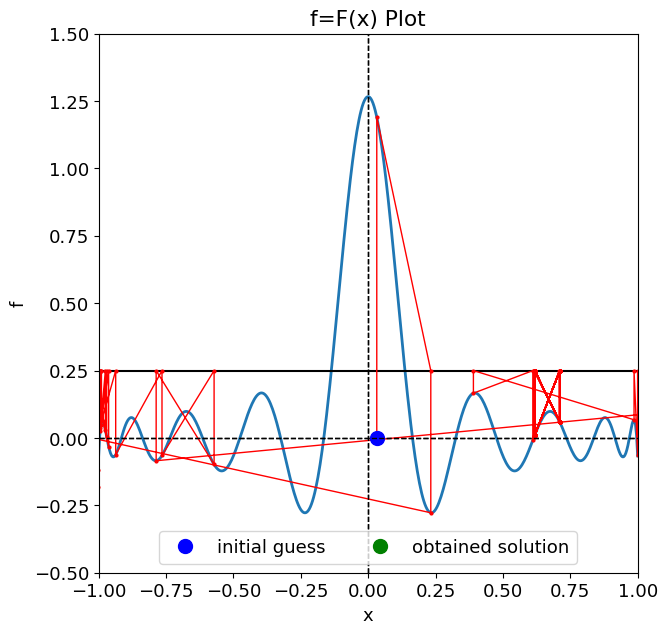
\includegraphics[width=\textwidth]{Figures/prob2_sol22.png}
        \end{block}
    \end{columns}
\end{frame}

\begin{frame}{Problem 2}{Observations}
    \begin{columns}
        \column{0.9\textwidth}
        \begin{block}{\footnotesize Observations made from previous test cases}
            \begin{enumerate}
                \footnotesize
                \item At f=0.0001 for any value of initial guess $x_0$, the solution converges except for the 'x' values corresponding to peaks.
                \item At f=0.25, similar to the problem 1, the convergence of the solution most probably will occur when the initial guess is in the neighborhood of the solution. Otherwise, it may or may not converge.
            \end{enumerate}
        \end{block}
    \end{columns}
\end{frame}

\begin{frame}{Problem 2}{Plotting the solution curve, $f\in[-0.5,1.5]$}
    \vspace{-2.5em}
    \begin{columns}
        \column[t]{0.5\textwidth}
        \begin{block}{\scriptsize For a single initial guess}
            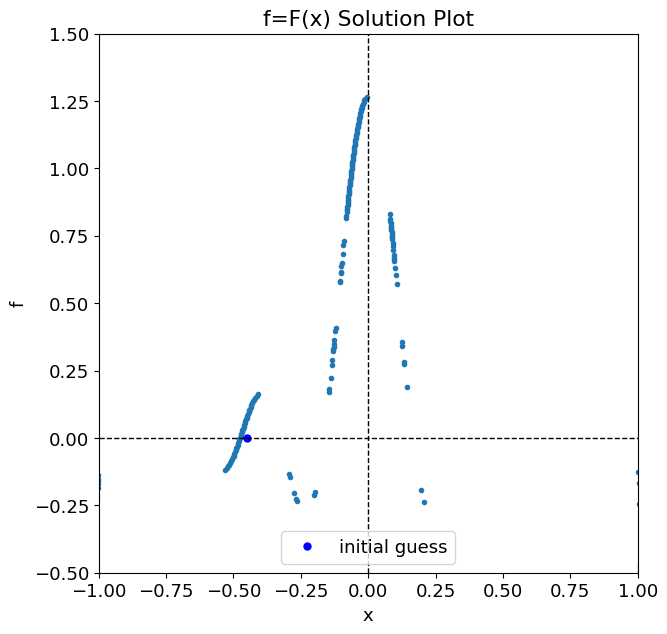
\includegraphics[width=\textwidth]{Figures/prob2_pltsol1.png}
        \end{block}
        \column[t]{0.43\textwidth}
        \begin{block}{\footnotesize Observations }
            \footnotesize
            \begin{itemize}
                \item For a grid of 1000 points on 'f' axis, and with an arbitrary initial guess the graph plotted gives an incomplete description of the nonlinear function.
            \end{itemize}
        \end{block}
    \end{columns}
\end{frame}

\begin{frame}{Problem 2}{Plotting the solution curve, $f\in[-0.5,1.5]$}
    \vspace{-2.5em}
    \begin{columns}
        \column[t]{0.5\textwidth}
        \begin{block}{\scriptsize For multiple initial guesses - combined plot }
            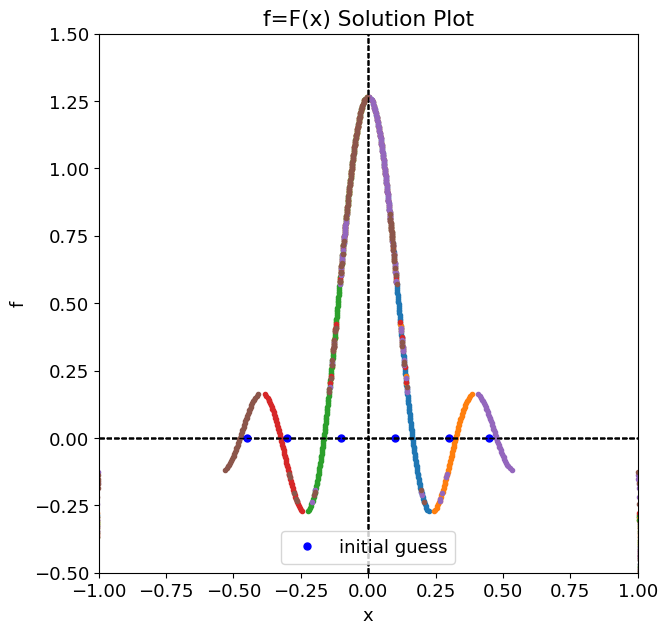
\includegraphics[width=\textwidth]{Figures/prob2_pltsol2.png}
        \end{block}
        \column[t]{0.43\textwidth}
        \begin{block}{\footnotesize Observations }
            \footnotesize
            \begin{itemize}
                \item For a grid of 1000 points on 'f' axis, and with an arbitrary initial guess the graph plotted gives an incomplete description of the nonlinear function.
                \item But, in contrast to problem 1, instead of choosing initial guess in such a way that it gives a monotonic section of the graph, one can also take multiple random initial guesses and combine all the obtained data points to get the complete description of the nonlinear function.
            \end{itemize}
        \end{block}
    \end{columns}
\end{frame}

%===================================================================
\section{System of equations}

\begin{frame}{System of equations}{2 equations - decoupled}
    \vspace{-2em}
    \begin{columns}[t]
        \column{0.5\textwidth}
        \begin{block}{\footnotesize Procedure}
            \scriptsize
            Let $\mathcal{F}(\textbf{x})=0$ be a system of nonlinear equations
            \[
                F_1 =\frac{x_1}{\sin x_1} - f_1 = 0 ,\quad F_2 =\frac{x_2}{\sin x_2} - f_2 = 0
            \]
            The solution is obtained using the directional derivative.
            \vspace{-1em}
            \[\implies D\ \mathcal{F}(\textbf{x}^k)[\textbf{u}]=-\mathcal{F}(\textbf{x}^k)\]
            \[\implies \frac{\partial\mathcal{F}(\textbf{x}^k)}{\partial \textbf{x}}\textbf{u}=-\mathcal{F}(\textbf{x}^k)\]
            \[
                \begin{bmatrix}
                    \frac{\partial F_1(x_1,x_2)}{\partial x_1} & \frac{\partial F_1(x_1,x_2)}{\partial x_2} \\
                    \frac{\partial F_2(x_1,x_2)}{\partial x_1} & \frac{\partial F_2(x_1,x_2)}{\partial x_2}
                \end{bmatrix}
                \begin{bmatrix}
                    u_1 \\ u_2
                \end{bmatrix}
                =
                \begin{bmatrix}
                    -F_1(x_1,x_2) \\
                    -F_2(x_1,x_2) 
                \end{bmatrix}
            \]
            \[
                \implies
                \begin{bmatrix}
                    \frac{\partial F_1}{\partial x_1} & 0 \\
                    0 & \frac{\partial F_2}{\partial x_2}
                \end{bmatrix}
                \begin{bmatrix}
                    u_1 \\ u_2
                \end{bmatrix}
                =
                \begin{bmatrix}
                    -F_1(x_1) \\
                    -F_2(x_2) 
                \end{bmatrix}
            \]
            \[\textbf{x}^{k+1}=\textbf{x}^k+\textbf{u}\]
        \end{block}
        \column{0.45\textwidth}
        \begin{block}{\footnotesize Example}
            \scriptsize
            \[
                F_1 =\frac{x_1}{\sin x_1} - 1.2 = 0
            \]
            \[
                F_2 =\frac{x_2}{\sin x_2} - 1.5 = 0
            \]
            For initial guess
            \vspace{-1em}
            \[
                \begin{bmatrix}
                    x_1^o \\ x_2^o
                \end{bmatrix}
                =
                \begin{bmatrix}
                    2.5 \\ 2.5
                \end{bmatrix}
            \]
            The solution at iteration 200
            \vspace{-0.8em}
            \[
                \begin{bmatrix}
                    x_1 \\ x_2
                \end{bmatrix}
                =
                \begin{bmatrix}
                    1.02673829 \\ 1.49578157
                \end{bmatrix}
                % \begin{matrix}
                %     \rightarrow & \text{converged} \\
                %     \rightarrow & \text{not converged}
                % \end{matrix}
            \]
            % \[
            %     \text{error} = 
            %     \begin{bmatrix}
            %         0.00000009 \\
            %         14.63783779
            %     \end{bmatrix}
            % \]

            % Therefore, the algorithm is able to predict both the converging and non-converging cases.
            The solution is matching with the solutions obtained form the problem 1.
        \end{block}
        \vfill
    \end{columns}
\end{frame}

\begin{frame}{System of equations}{2 equations - coupled}
    \vspace{-2em}
    \begin{columns}[t]
        \column{0.5\textwidth}
        \begin{block}{\footnotesize Example - 1}
            \scriptsize
            Let $\mathcal{F}(\textbf{x})=0$ be a system of nonlinear equations
            \[F_1 = x_1^{2}+2x_1x_2+x_2+4=0\]
            \vspace{-2em}
            \[F_2 = x_2^{2}+6x_1x_2+x_1^{2}+6=0\]
            \[
                \begin{bmatrix}
                    \frac{\partial F_1(x_1,x_2)}{\partial x_1} & \frac{\partial F_1(x_1,x_2)}{\partial x_2} \\
                    \frac{\partial F_2(x_1,x_2)}{\partial x_1} & \frac{\partial F_2(x_1,x_2)}{\partial x_2}
                \end{bmatrix}
                \begin{bmatrix}
                    u_1 \\ u_2
                \end{bmatrix}
                =
                \begin{bmatrix}
                    -F_1(x_1,x_2) \\
                    -F_2(x_1,x_2) 
                \end{bmatrix}
            \]
            \[\textbf{x}^{k+1}=\textbf{x}^k+\textbf{u}\]
            For initial guess
            \vspace{-1em}
            \[
                \begin{bmatrix}
                    x_1^o \\ x_2^o
                \end{bmatrix}
                =
                \begin{bmatrix}
                    2.5 \\ 2.5
                \end{bmatrix}
            \]
            The solution
            \vspace{-1em}
            \[
                \begin{bmatrix}
                    x_1 \\ x_2
                \end{bmatrix}
                =
                \begin{bmatrix}
                    -1.0370868 \\ 4.72507334
                \end{bmatrix}
            \]
            Number of iterations = 8
        \end{block}
        \column{0.45\textwidth}
        \begin{block}{\footnotesize Example Plot - 1}
            \scriptsize
            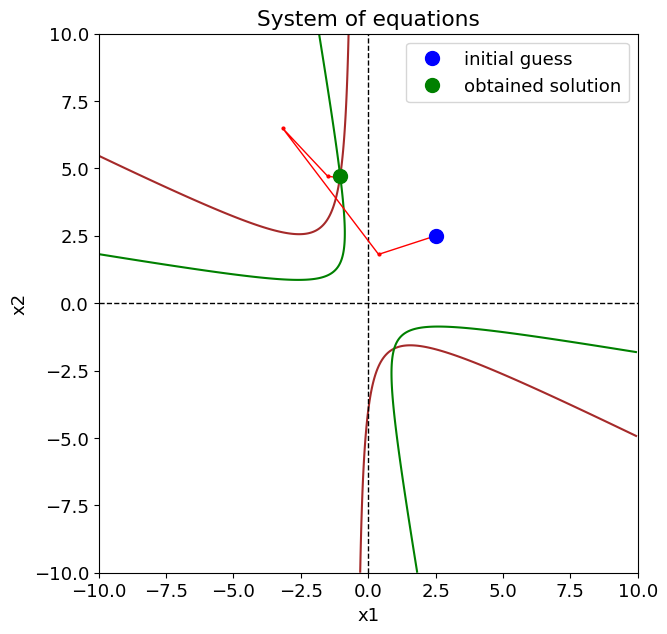
\includegraphics[width=\textwidth]{Figures/syseqns_1.png}
        \end{block}
        \vfill
    \end{columns}
\end{frame}

\begin{frame}{System of equations}{2 equations - coupled}
    \vspace{-2em}
    \begin{columns}[t]
        \column{0.5\textwidth}
        \begin{block}{\footnotesize Example - 2}
            \scriptsize
            Let $\mathcal{F}(\textbf{x})=0$ be a system of nonlinear equations
            \[F_1 = x_1^{2}+2x_1x_2+x_2+4=0\]
            \vspace{-2em}
            \[F_2 = x_2^{2}+6x_1x_2+x_1^{2}+6=0\]
            \[
                \begin{bmatrix}
                    \frac{\partial F_1(x_1,x_2)}{\partial x_1} & \frac{\partial F_1(x_1,x_2)}{\partial x_2} \\
                    \frac{\partial F_2(x_1,x_2)}{\partial x_1} & \frac{\partial F_2(x_1,x_2)}{\partial x_2}
                \end{bmatrix}
                \begin{bmatrix}
                    u_1 \\ u_2
                \end{bmatrix}
                =
                \begin{bmatrix}
                    -F_1(x_1,x_2) \\
                    -F_2(x_1,x_2) 
                \end{bmatrix}
            \]
            \[\textbf{x}^{k+1}=\textbf{x}^k+\textbf{u}\]
            For initial guess
            \vspace{-1em}
            \[
                \begin{bmatrix}
                    x_1^o \\ x_2^o
                \end{bmatrix}
                =
                \begin{bmatrix}
                    0.00001 \\ 0.00001
                \end{bmatrix}
            \]
            The solution
            \vspace{-1em}
            \[
                \begin{bmatrix}
                    x_1 \\ x_2
                \end{bmatrix}
                =
                \begin{bmatrix}
                    0.96774125 \\ -1.6816735
                \end{bmatrix}
            \]
            Number of iterations = 25
        \end{block}
        \column{0.45\textwidth}
        \begin{block}{\footnotesize Example Plot - 2}
            \scriptsize
            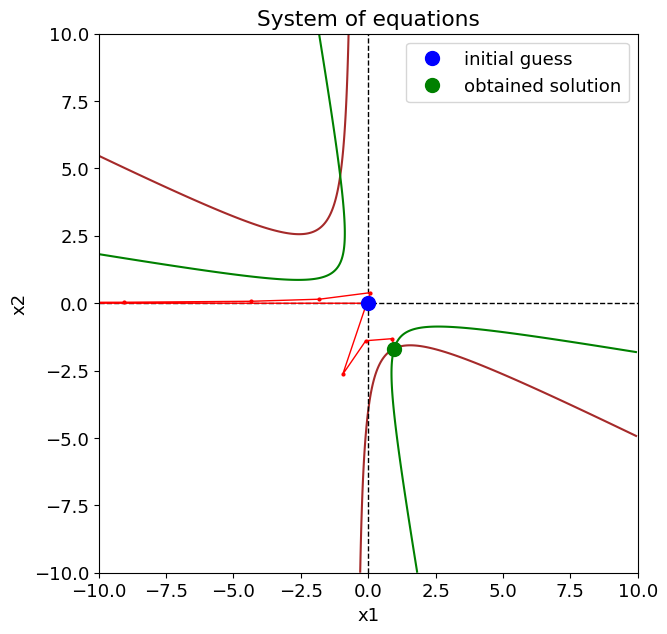
\includegraphics[width=\textwidth]{Figures/syseqns_2.png}
        \end{block}
        \vfill
    \end{columns}
\end{frame}

\begin{frame}{System of equations}{2 equations - coupled}
    \vspace{-2em}
    \begin{columns}[t]
        \column{0.5\textwidth}
        \begin{block}{\footnotesize Example - 3}
            \scriptsize
            Let $\mathcal{F}(\textbf{x})=0$ be a system of nonlinear equations
            \[F_1 = x_1^{2}+2x_1x_2+x_2+4=0\]
            \vspace{-2em}
            \[F_2 = x_2^{2}+6x_1x_2+x_1^{2}+6=0\]
            \[
                \begin{bmatrix}
                    \frac{\partial F_1(x_1,x_2)}{\partial x_1} & \frac{\partial F_1(x_1,x_2)}{\partial x_2} \\
                    \frac{\partial F_2(x_1,x_2)}{\partial x_1} & \frac{\partial F_2(x_1,x_2)}{\partial x_2}
                \end{bmatrix}
                \begin{bmatrix}
                    u_1 \\ u_2
                \end{bmatrix}
                =
                \begin{bmatrix}
                    -F_1(x_1,x_2) \\
                    -F_2(x_1,x_2) 
                \end{bmatrix}
            \]
            \[\textbf{x}^{k+1}=\textbf{x}^k+\textbf{u}\]
            For initial guess
            \vspace{-1em}
            \[
                \begin{bmatrix}
                    x_1^o \\ x_2^o
                \end{bmatrix}
                =
                \begin{bmatrix}
                    -10 \\ -10
                \end{bmatrix}
            \]
            The solution
            \vspace{-1em}
            \[
                \begin{bmatrix}
                    x_1 \\ x_2
                \end{bmatrix}
                =
                \begin{bmatrix}
                    0.96774125 \\ -1.6816735
                \end{bmatrix}
            \]
            Number of iterations = 10
        \end{block}
        \column{0.45\textwidth}
        \begin{block}{\footnotesize Example Plot - 3}
            \scriptsize
            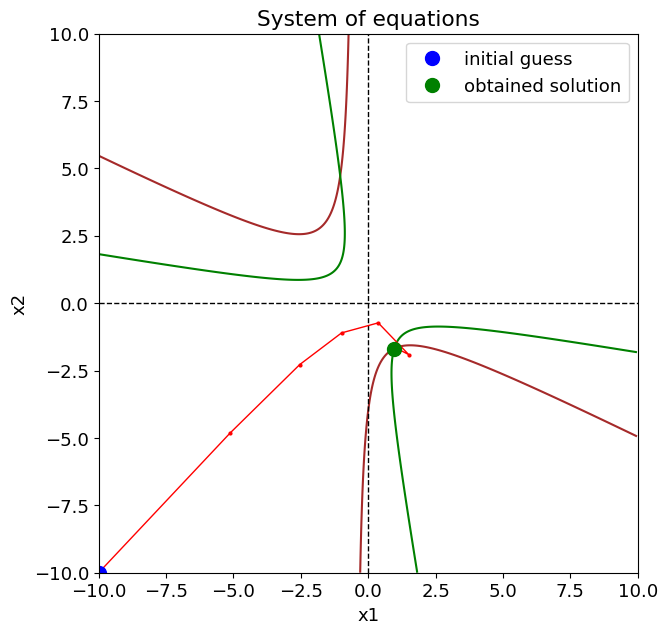
\includegraphics[width=\textwidth]{Figures/syseqns_3.png}
        \end{block}
        \vspace{-0.7em}
        \begin{block}{\footnotesize Observations}
            \scriptsize
            The algorithm is able to predict one of the existing solutions based on the initial guess.
        \end{block}
    \end{columns}
\end{frame}

%===================================================================
\section{Conclusions}

\begin{frame}[t]{Conclusions}{Observations made from the used solution algorithms}
        \begin{block}{\footnotesize Single-variable nonlinear equations}
            \footnotesize
            \begin{enumerate}
                \item In case of single-variable nonlinear equations, when the initial guess is in the neighborhood of the solution, convergence will most probably occur. Otherwise, convergence may or may not occur depending on the nonlinear behavior of the function.
                \item The complete description of the behavior of the function is not possible with the data points obtained from one initial guess (since it is a nonlinear function). Instead, the combined plot obtained using multiple initial guesses can describe the function completely.
            \end{enumerate}
        \end{block}
        \begin{block}{\footnotesize System of nonlinear equations}
            \footnotesize
            \begin{enumerate}
                \item The algorithm is able to predict any one of the solutions (if there exists multiple) which depends on the initial guess.
            \end{enumerate}
        \end{block}
\end{frame}

% %---------------------SLIDE---------------------------------------
% \begin{frame}{Equations of motion} 
% \begin{columns}
%     \column{0.4\textwidth}
%     \begin{block}{Newton's second law}
%    $m\ddot{x} = F(\dot{x}, x, t)$
%     \end{block}
%     \begin{block}{Schrödinger's equation}
%     ${\displaystyle i\hbar {\frac {d}{dt}}\vert \Psi (t)\rangle ={\hat {H}}\vert \Psi (t)\rangle }$
%     \end{block}
%     \begin{block}{Ampère's circuital law}
%     $ \nabla \times \mathbf{B}=\frac{1}{c}\left(4 \pi \mathbf{J}+\frac{\partial \mathbf{E}}{\partial t}\right)$
%     \end{block}
% \end{columns}
% \end{frame}
% %---------------------SLIDE---------------------------------------
% \begin{frame}{Important question}
%     Important question again
% \end{frame}
% %---------------------SLIDE---------------------------------------
% \section{Important section}
% \begin{frame}{Bullet points}
% \begin{itemize}
%     \item Item A
%     \item Item B
%     \item Item C
% \end{itemize}
% \end{frame}
% %---------------------SLIDE---------------------------------------
% \begin{frame}{Using pause}
% This is a sentence. \pause 
% And this too. \pause
% \alert{Bye}. 
% \end{frame}

% %---------------------SLIDE--------------------------------------
% \begin{frame}{A Theorem}
% \begin{theorem}[Freshman's Dream] 
%  $(a+b)^p \equiv a^p + b^p \, (mod \,p)$ if p is a prime number.
% \end{theorem} \pause
% \begin{proof}
% A valid proof.
% \end{proof}
% \begin{example}
% Maybe an example?
% \end{example}
% \end{frame}

% %-----------------------------SLIDE --------------------------------------

% %Below must be compiled using LuLaTex (for emoji package):

% % \begin{frame}{Summary}

% % \begin{itemize}
% %     \item[\emoji{check-mark-button}] Concept A
% %      \item[\emoji{check-mark-button}] Concept B
% %      \item[\emoji{check-mark-button}] Concept C
% % \end{itemize}
% % \end{frame}


% %-----------------------------SLIDE --------------------------------------

% \begin{frame}{How do you write a thesis?}

% \begin{enumerate}
%     \item Eat
%     \item Sleep
%     \item Rave
%     \item Repeat
% \end{enumerate}
% \end{frame}


% %-----------------------------SLIDE --------------------------------------

% \begin{frame}{Frame title}{Frame subtitle}
% This is how you can cite \cite{Dirac}.
% \end{frame}
% %-----------------------------SLIDE --------------------------------------
% \begin{frame}{The end.}
% \begin{columns}
% \column{0.4\textwidth}
% This is a column.

% \column{0.4\textwidth}
% 
\includegraphics[width=0.9\textwidth]{Figures/meme.png}    
% \end{columns}    
    
    
% \end{frame}

% %---------------------------------------------------------
% \section{References}
% \begin{frame}[allowframebreaks]\frametitle{References}
%         \bibliographystyle{apalike}
%         \bibliography{bib}
% \end{frame}


\end{document}